%\title{relatório SO2}
%----------------------------------------------------------------------------------------
%	PACKAGES AND OTHER DOCUMENT CONFIGURATIONS
%----------------------------------------------------------------------------------------

\makeindex
\documentclass[a4paper,12pt,headings=small]{article}
\usepackage[portuguese]{babel}
\usepackage[export]{adjustbox}
\usepackage[utf8x]{inputenc}
\usepackage{amsmath}
\usepackage{graphicx}
\usepackage{hyperref}
\usepackage{url}
\usepackage[colorinlistoftodos]{todonotes}
\usepackage{placeins}
\usepackage{makeidx}
\usepackage[left=2.5cm,right=2.5cm,top=2.5cm,bottom=2.5cm,a4paper]{geometry}
\usepackage{blindtext}
\usepackage{listings}
\usepackage{float}
\setlength\footskip{1cm}

\begin{document}

\begin{titlepage}

\newcommand{\HRule}{\rule{\linewidth}{0.5mm}} % Defines a new command for the horizontal lines, change thickness here

\center % Center everything on the page




 %----------------------------------------------------------------------------------------
%	LOGO SECTION
%----------------------------------------------------------------------------------------


\includegraphics[scale=1]{uelogo.png}\\[0.5cm] 

%----------------------------------------------------------------------------------------
 
%----------------------------------------------------------------------------------------
%	HEADING SECTIONS
%----------------------------------------------------------------------------------------

\textsc{\Large Linguagens de Programação}\\[1cm]


%----------------------------------------------------------------------------------------
%	TITLE SECTION
%----------------------------------------------------------------------------------------

\HRule \\[0.4cm]
{ \huge \bfseries Relatório do primeiro trabalho prático}\\[0.4cm] 
\HRule \\[1 cm]
 
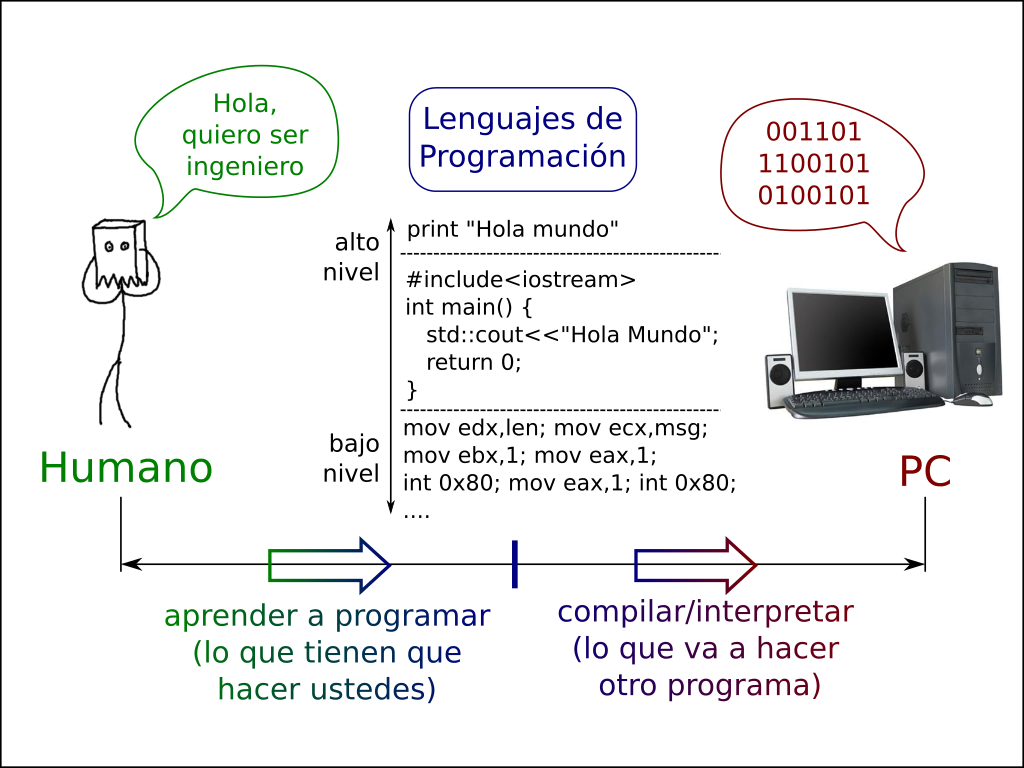
\includegraphics[scale=0.3]{lp.png}\\[0.5cm] 

%----------------------------------------------------------------------------------------
%	AUTHOR SECTION
%----------------------------------------------------------------------------------------
%
\begin{minipage}{0.4\textwidth}
\begin{flushleft} \large
\emph{Autores:}\\
João \textsc{Marques}, 39996\\
Tiago \textsc{Martinho}, 35735\\
\end{flushleft}
\end{minipage}
~
\begin{minipage}{0.4\textwidth}
\begin{flushright} \large
\emph{Docente:} \\
Teresa \textsc{Gonçalves} \\
\end{flushright}
\end{minipage}\\[2cm]


%----------------------------------------------------------------------------------------
%	DATE SECTION
%----------------------------------------------------------------------------------------
{\large Maio de 2020}\\[1cm]  

\vfill % Fill the rest of the page with whitespace

\end{titlepage}

\newpage
\thispagestyle{empty}
\renewcommand\contentsname{Índice}
\tableofcontents
\newpage

\printindex

\section{Introdução}
\FloatBarrier
No âmbito da unidade curricular de Linguagens de Programação, pretende-se implementar uma máquina \textbf{TISC}. Nesta primeira fase do trabalho pretende-se desenvolver a \textbf{memória de instruções}, \textbf{pilha de avaliação}, \textbf{gestor de etiquetas} e \textbf{memória de instruções}.\\
Este trabalho foi desenvolvido na linguagem de progamação \textit{Java} usando as biblotecas \textit{JLex} e \textit{JCup}.\\
Esta implementação da máquina \textbf{TISC} tem como objectivo simular e funcinar como um intrepetador de TISC.

\section{Instruções}
Decidiu-se que a melhor maneira de tratar das instruções seria criar uma classe \textit{\textbf{Instruction}} e 7 subclasses, uma para cada tipo diferente de instrução.\\

\begin{itemize}
\item Instruções aritméticas
\item Instruções para manipulação de inteiros
\item Instruções de acesso a variáveis
\item Instruções de acesso a argumentos
\item Instruções para chamada de funções
\item Instruções de salto
\item Instruções de saída
\end{itemize}

\section{Desenvolvimento}

\subsection{Memória de instruções}
\FloatBarrier
A memória das instruções irá funcionar como uma lista iterada das instruções. Para tal utilizou-se um \textit{Vector} uma vez que tem dimensões dinâmicas e pode ser facilmente iterado (noutra fase pelo PC).\\
Este vector está parameterizado para objectos do tipo \textit{Instruction}.

\subsection{Pilha de avaliação}
\FloatBarrier
A pilha de avaliação, neste momento do trabalho, usou-se uma \textit{Stack}.

\subsection{Gestor de etiquetas}
\FloatBarrier
Para gerir as etiquetas utilizou-se um \textit{HashMap} uma vez que se pretende saber o índice da instrução (PC) a qual a etiqueta corresponde.

\subsection{Memória de instruções}
\FloatBarrier
Como esta parte ainda não foi aprofundada neste trabalho optou-se por um \textit{Vector} uma vez que se pretende que funcione como uma lista.

\section{Execução}
Para compilar deve-se utilizar o \textit{Makefile} fazendo \textit{make}.\\
Nesta fase do trabalho apenas se imprime no \textit{stdout} a memória de instruções.

\end{document}


